\chapter{MiCS User Manual}
\label{chap:mics_manual}
MiCS is a framework for ASP.NET Web Forms that makes it possible to write JavaScript safely by translating C\# to JavaScript. This approach also makes it possible to execute the same code both on server and client side and it ensures consistency between JavaScript code and HTML elements.

This chapter demonstrates how to use MiCS. The manual will illustrate how to write server side code that can be reused on client side in a safe manner. It is assumed that the developer uses Visual Studio and .NET 4.0. In this manual a simple registration form, shown in figure \ref{fig:manual_registrationform}, is created. The code is explained step-by-step but can also be found in its entirety in Appendix \ref{AppendixA}.

\begin{figure}[H]
	\begin{center}
		\centerline{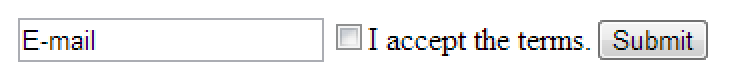
\includegraphics[width=12cm]{resources/images/manual_registrationform.png}}
	\end{center}
	\caption{Simple e-mail registration form.}
	\label{fig:manual_registrationform}
\end{figure}


\subsubsection{1. MiCS-enable Your Web Application} % (fold)
\label{ssub:mics_enable_your_web_application}
Create a new ASP.NET Web Application and add a reference to the MiCS.dll. Goto the \texttt{Default.aspx.cs} Code Behind file and add using statements for \texttt{System.Html}, which contains all the ClientSide DOM types and \texttt{MiCS}. Change the \texttt{Default} class to inherit from \texttt{MiCSPage} instead of \texttt{System.Web.UI.Page}. See figure \ref{fig:mics_enable_web_application}.
\begin{figure}[H]
\begin{lstlisting}[language=CSharp,classoffset=1,morekeywords={Default,MiCSPage,Button,CheckBox,TextBox,EventArgs,ClientSide,InputElement,Document,CheckBoxElement,Window,MixedSide,Regex}]
...
using MiCS;
using System.Html;

namespace MiCSManual
{
    public partial class Default : MiCSPage
    {
        protected void Page_Load(object sender, EventArgs e)
        {
   
        }
    }
}
\end{lstlisting}
\caption{MiCS enabled Default.aspx.cs Code Behind file}
\label{fig:mics_enable_web_application}
\end{figure}
% subsubsection mics_enable_your_web_application (end)

Add the relevant Web Controls to the page, as shown in figure \ref{fig:mics_add_controls}

\begin{figure}[H]
\begin{lstlisting}[language=CSharp,classoffset=1,morekeywords={Default,MiCSPage,Button,CheckBox,TextBox,EventArgs,ClientSide,InputElement,Document,CheckBoxElement,Window,MixedSide,Regex}]
...

public partial class Default : MiCSPage
{
  Button button;
  CheckBox checkBox;
  TextBox emailBox;

  protected void Page_Load(object sender, EventArgs e)
  {
    emailBox = new TextBox() { ID = "EmailBox", Text = "E-mail" };
    checkBox = new CheckBox() { ID = "CheckBox", Text = "I accept the terms."};
    button = new Button() { Text = "Submit" };

    form1.Controls.Add(emailBox);
    form1.Controls.Add(checkBox);
    form1.Controls.Add(button);
  }
}

...
\end{lstlisting}
\caption{Add simple registration form controls from Code Behind}
\label{fig:mics_add_controls}
\end{figure}
% subsubsection mics_enable_your_web_application (end)



\subsubsection{2. Writing MiCS Code} % (fold)
\label{ssub:writing_mics_code}
It is now possible to write code that can be used both on server side and client side. This is done by adding the \texttt{MixedSide} attribute to a method, as shown in figure \ref{fig:write_mics_code}

\begin{figure}[H]
\begin{lstlisting}[language=CSharp,classoffset=1,morekeywords={Default,MiCSPage,Button,CheckBox,TextBox,EventArgs,ClientSide,InputElement,Document,CheckBoxElement,Window,MixedSide,Regex}]
...
using System.Text.RegularExpressions;

namespace MiCSManual
{    
  public partial class Default : MiCSPage
  {
    ...

    [MixedSide]
    bool IsEmailValid(string email)
    {
      var emailRegex = new Regex("^[A-z0-9._%+-]+@[A-z0-9.-]+.[A-z]{2,4}$");
      return emailRegex.IsMatch(email);
    }
  }
}
\end{lstlisting}
\caption{An e-mail validation function that can be used both on server and client side.}
\label{fig:write_mics_code}
\end{figure}

Code that is only intended for use on client side, can be written in a similar manner, but by adding the \texttt{ClientSide} attribute to the method. In figure \ref{fig:write_mics_code_clienside} a button click event handler is created. The method is supposed to run on client side when the submit button is clicked. Notice how the method makes use of the mixed side \texttt{isEmailValid} method.


\begin{figure}[H]
\begin{lstlisting}[language=CSharp,classoffset=1,morekeywords={Default,MiCSPage,Button,CheckBox,TextBox,EventArgs,ClientSide,InputElement,Document,CheckBoxElement,Window,MixedSide,Regex}]
[ClientSide]
bool button_ClientClick()
{
  var emailField = (InputElement)Document.GetElementById("EmailBox");
  var termsCheckBox = (CheckBoxElement)Document.GetElementById("CheckBox");
  
  if (!isEmailValid(emailField.Value))
  {
    Window.Alert("Invalid E-mail!");
    return false;
  }
  
  if (!termsCheckBox.Checked)
  {
    Window.Alert("Accepting terms are required!");
    return false;
  }
  
  return true;
}
\end{lstlisting}
\caption{Client side only method that calls the \texttt{IsEmailValid} mixed side method. Both methods resides on the \texttt{Default} class.}
\label{fig:write_mics_code_clienside}
\end{figure}
% subsubsection writing_mics_code (end)

\subsubsection{3. Register Click Events} % (fold)
\label{ssub:3_register_click_events}
	The last thing that needs to be done is registering click events on the submit button, both for the client and server side. Web Controls, like buttons, also have server side events in ASP.NET Web Forms. Registering click events is done as the last thing in the \texttt{Page\_Load} event as shown in figure \ref{fig:register_events}. Note that the server side click event handler is also defined here.
\begin{figure}[H]
\begin{lstlisting}[language=CSharp,classoffset=1,morekeywords={Default,MiCSPage,Button,CheckBox,TextBox,EventArgs,ClientSide,InputElement,Document,CheckBoxElement,Window,MixedSide,Regex}]
protected void Page_Load(object sender, EventArgs e)
{
  ...

  // Register the server side click event
  button.Click += button_Click;

  // Register the client side click event
  button.OnClientClick(button_ClientClick);
}

void button_Click(object sender, EventArgs e)
{
  if (isEmailValid(emailBox.Text) && checkBox.Checked)
    form1.Controls.Add(new Label() { Text = "Registration Complete." });
  else
    form1.Controls.Add(new Label() { Text = "Server Side Registration Failed!" });
}
...
\end{lstlisting}
\caption{Registration of both server and client side button click events.}
\label{fig:register_events}
\end{figure}

% subsubsection 3_register_click_events (end)

Now the example web application can be run. If the client side validation passes, the form is submitted and validated on server side as well.

If the user does not enter a valid e-mail address or doesn't accept the terms, he will be alerted with an error message and the form will not submit. Should the user bypass the client side validation, the server side validation will step in, and the user will be met with an error message generated from server side instead.

The generated HTML and JavaScript source code is shown in Figure \ref{fig:manualHtmlSource}.

\begin{figure}[H]
\begin{lstlisting}[language=html,style=HTMLJSStyle]
<!DOCTYPE html>
<html xmlns="http://www.w3.org/1999/xhtml">
<head><title></title></head>
<body>
    <form method="post" action="./" id="form1">
    ...
    <script type="text/javascript">
    //<![CDATA[
    function MiCSManual$Default() {
    }
    MiCSManual$Default.prototype = {
      button_ClientClick: function() {
        var emailField = document.getElementById('EmailBox');
        var termsCheckBox = document.getElementById('CheckBox');
        if (!this.isEmailValid(emailField.value)) {
          window.alert('Invalid E-mail!');
          return false;
        }
        if (!termsCheckBox.checked) {
          window.alert('Accepting terms are required!');
          return false;
        }
        return true;
      },
      isEmailValid: function(email) {
        var emailRegex = new RegExp('^[A-z0-9._%+-]+@[A-z0-9.-]+.[A-z]{2,4}$');
        return emailRegex.test(email);
      }
    };
    //]]>
    </script>
    ...
    <input name="EmailBox" type="text" value="E-mail" id="EmailBox">
    <input id="CheckBox" type="checkbox" name="CheckBox">
    <label for="CheckBox">I accept the terms.</label>
    <input type="submit" name="ctl03" value="Submit" 
     onclick="var obj = new MiCSManual$Default(); return obj.button_ClientClick();">
    </form>
</body>
</html>
\end{lstlisting}
\caption{The manual example's resulting HTML source code.}
\label{fig:manualHtmlSource}
\end{figure}

In this simple registration form example we have now essentially written JavaScript in a safe manner, we have reused server side code on client side and we have ensured consistency between HTML and JavaScript by registering the client side click event in a safe (compile time validated) manner.

